\documentclass[headsepline]{scrreprt}

\usepackage[utf8]{inputenc}
\usepackage{csquotes}
\usepackage[english]{babel}


\usepackage{scrlayer-scrpage}
\pagestyle{scrheadings}
\automark[section]{section}
\clearpairofpagestyles
\ohead{\headmark}
\ofoot[\pagemark]{\pagemark}

\usepackage[]{graphicx}
\graphicspath{{gfx/}}
\DeclareGraphicsExtensions{.png,.jpg,.pdf}

\usepackage{amsfonts}
\usepackage{amsmath}
\usepackage{hyperref}

\usepackage{algorithm,algorithmicx,algpseudocode}

\newcommand{\handindate}{xx.xx.2022}

\usepackage[backend=biber, style=alphabetic, maxcitenames=2]{biblatex}
\addbibresource{bibliography.bib}

\begin{document}
\thispagestyle{empty}

{\sffamily
	\begin{figure}
		
\includegraphics[height=20mm]{logo_luh}
		\hfill
		
\includegraphics[height=20mm]{l3s_logo}
	\end{figure}
	\begin{center}
		\mbox{} \\
		\vspace{1.5cm}
		\huge{Deconstructing Ranking Abilities of

			Language Models}\\
		\vspace{1.8cm}
		{\large
			Gottfried Wilhelm Leibniz Universität Hannover\\
			Fakultät für Elektrotechnik und Informatik\\
			Institut für verteilte Systeme \\
			Fachgebiet Wissensbasierte Systeme \\
			Forschungszentrum L3S \\
			\vspace{1.8cm}
			Thesis by \\
			\textbf{Fabian Beringer} \\
			\vspace{1.8cm}
			\begin{tabular}{rl}
				First examiner:  & Prof. Dr. Wolfgang Nejdl \\
				Second examiner: & Dr. Sowmya S. Sundaram   \\
				Advisor:         & Jonas Wallat             \\
			\end{tabular}
			\vfill
			Hannover, \handindate
		}
	\end{center}
}
\newpage

\chapter*{Abstract}
...

\tableofcontents

\chapter{Introduction}
general retrieval ?
\section{Motivation}
Over the last couple of years, contextualized language representations from deep neural network (DNN) models have become the go-to approach for tackling natural language processing (NLP) tasks. In particular, the \ti{transformer} \cite{vaswani2017attention} and its variants, combined with large-scale, unsupervised pre-training, have shown unprecedented performance in a variety of NLP benchmarks.

However, unlike traditional approaches, these models consist of billions of automatically learned parameters, effectively turning them into huge black box functions. Because of this, understanding why and how such a model arrives at a certain decision, becomes a challenge in itself. Yet, as more and more NLP systems rely on these kinds of models, gaining a better understanding of their internal workings becomes crucial, especially when facing problems such as learned social biases \cite{Nadeem2021StereoSetMS,Bender2021OnTD, kurita2019measuring}, falsely motivated predictions \cite{10.1145/2939672.2939778, DBLP:journals/corr/abs-1802-00614} or simply trying to determine causes of prediction error. In addition, a better understanding might provide insights on model weaknesses and guide model improvement, e.g. when adapting to new domains.

Recent work on understanding neural language models has aimed at measuring the extent, to which certain knowledge is encoded in word representations. For this, a \ti{probing} classifier or \ti{probe} is trained on these representations given a language task. The probe's performance is then expected to reflect how well the representations capture the knowledge required for solving that task.

has recently emerged for nlp, but retrieval which important: google guides how we access information etc

we look at bert, initial break through approach, more recent iterations still similar in essence

\section{Problem Statement}
research question:
\begin{itemize}
    \item given set of tasks, presumably ranking related, which knowledge does bert encode?
    \item how does ranking trained model differ from base language model
    \item can we exploit these differences to inform training for ranking?
\end{itemize}
\section{Contribution}

\section{Thesis Outline}

\chapter{Foundations}
\label{foundations}
\section{Information Retrieval - Ranking Text}
Ranking is an integral part of the information retrieval (IR) process. The general IR problem can be formulated as follows: A user with a need for information expresses this information need through formulation of a query. Now given the query and a collection of documents, the IR system's task is to provide a list of documents that satisfy the user's information need. Further, the retrieved documents should be sorted by relevance w.r.t. the user's information need in descending order, i.e. the documents considered most relevant should be at the top of the list.

While from this formulation only, the task might appear simple, there are several caveats to look out for when it comes to ranking. For instance, there is no restriction on the structure of the query. While we might expect a natural language question like "What color are giraffes?" a user might decide to enter a keyword query like "giraffes color". The same applies to documents: Depending on the corpus we are dealing with, the documents might be raw text, structured text like HTML or even another type of media e.g. image, audio or a combination thereof.

Another possible issue is a mismatch in information need of the user and the corresponding query. Even if we find a perfect ordering of documents with respect to the query, we can not know for certain that the query actually reflects the user's information need. The user might not even know exactly what they're looking for until discovery through an iterative process, i.e. the information need is fuzzy and can not be specified through an exact query from the beginning on.

Further, a query might require additional context information in order for an IR system to find relevant documents. For example, depending on the time at which a query is prompted, the correct answer might change: "Who is president?" should return a different set of documents, as soon as a new president has been elected. Also, since not specified further, it is up to interpretation which country's president the user is interested in and might depend on their location.
In addition, even the corpus might not be static either and change or grow over time, e.g. web search has to deal with an ever-growing corpus: the internet.

While this list of issues is not comprehensive, at this point the complexity of the ranking problem should have become apparent.

Because this work focuses on the ranking of text in the context of web search, we will now give a formal definition with that scenario in mind:

Given a set of $|Q|$ natural language queries $Q = \{q_i\}_{i=1}^{|Q|}$ and a collection of $|D|$ documents $D = \{d_i\}_{i=1}^{|D|}$, we want to find a scoring function $s: Q \times D \rightarrow \mathbb{R}$, such that for any query $q \in Q$ and documents $d, d' \in D$, it holds true that $s(q, d) > s(q, d')$ if $d$ is more relevant w.r.t $q$ than $d'$.

To give the reader a more concrete idea and as we are going to build upon it throughout this work, we will now discuss two traditional approaches to text retrieval which, unlike neural retrieval, are based on exact matching, meaning query and document terms are compared directly. Further, they're "bag of word" models, meaning queries and documents are treated as sets of terms without considering order.

\subsection{TF-IDF}
Term Frequency - Inverted Document Frequency weighting (TF-IDF), is a traditional ranking approach that, given a query, assigns a relevance score to each document based on two assumptions:
\begin{enumerate}
    \item A document is relevant if terms from the query appear in it often.
    \item A document is relevant if the terms shared with the query are also rare in the collection.
\end{enumerate}

From these assumptions, two metrics are derived:
\begin{enumerate}
    \item Term-Frequency
          \begin{equation}
              w_{t,d} = \begin{cases}
                  1 + \log \text{tf}_{t, d} & \text{if } \text{tf}_{t, d} > 0 \\
                  0                         & \text{otherwise}                \\
              \end{cases}
          \end{equation}

          where $\text{tf}_{t, d}$ is the count of term $t$ in document $d$. The logarithmic scaling is motivated by the idea that a document does not linearly become more relevant by the number of terms in it: A document containing a term 10 times more often doesn't necessarily mean it is $10$ times more important, e.g. the document might just be very long and contain more words in general. Note that this is just one possible normalization scheme out of many.

    \item Inverted Document Frequency
          \begin{equation}
              \text{idf}(t, d) = \log \frac{|D|}{\text{df}_t}
          \end{equation}
          where $\text{df}_t$ counts the number of documents that a term occurs in over the full corpus. This way, terms that occur less frequent relative to the corpus size will receive a high IDF score and those that are more frequent a lower score.

\end{enumerate}

\begin{table}

\end{table}
To compute TF-IDF we can simply sum over the product of TF and IDF for each term in the query to produce a relevance score:
\begin{equation}
    \text{score}(q, d) = \sum_{t \in q} w_{t,d} \times \text{idf}_t
\end{equation}

Alternatively, vector space idf vector
\subsection{BM25}

\section{Machine Learning}
Machine learning can be described as a set of statistical methods, for automatically recognizing and extracting patterns from data. Typically, we can distinguish between two main types of machine learning: Supervised learning and unsupervised learning.

In the case of supervised learning, we have a set of training instances $X = \{x_i\}_{i=1}^N$ and corresponding labels $Y = \{y_i\}_{i=1}^N$, assigning a certain characteristic to each data point. For example, this characteristic might be a probability distribution over a set of classes or a regression score. If each $y_i$ represents one or more categories from a fixed set of classes $C = \{c_i\}_{i=1}^{|C|}$, this is called a classification problem.

Now given the training data and labels, the goal is to find a hypothesis that explains the data, such that for unseen data points $x' \notin X$, the labels $y' \notin Y$ can be inferred automatically. One way to estimate the generalization ability of a model or algorithm, is to divide the dataset into a training and a test set, and only train on the training set while using the test set for evaluation. If the test set models the full distribution of data adequately, it can act as a proxy for estimating the error on unseen samples.

In contrast, in unsupervised learning there is no access to any labels whatsoever. Characteristics of the data need to be learned solely from the data $X$ itself. Examples for this include clustering where $X$ is clustered into groups, representation learning which usually tries to find vector representations for $X$, as well as dimensionality reduction that, if each $X$ is already a vector, tries to compress them into more compact but still informative representations.

That being said, the separating lines between supervised and unsupervised learning are blurry. Especially with the emergence of semi-supervised approaches and "end2end" representation learning, modern ML methods often integrate parts of both.

\section{Deep Learning}
Deep learning is a subfield of ML that makes use of a class of models called Deep Neural Networks (DNN). Typically, DNNs find application in the supervised learning scenario and are often used for classification tasks. In the following we explain the basic mechanisms of DNNs and common approaches to train them.

\subsection{Deep Neural Networks}
In essence, a Deep Neural Network (DNN) is a function approximator $f: \mathbb{R}^n \rightarrow \mathbb{R}^m$ that applies a series of non-linear transformations to its inputs, in order to produce an output. In its simplest form, an input vector $x \in \mathbb{R}^n$ is multiplied by a single weight matrix, a bias vector is added, and the resulting vector is passed through a non-linear activation function $\sigma$.

\begin{equation}
    f(x) = \sigma(W x + b)
\end{equation}

where $W \in \mathbb{R}^{m \times n}$ and $b \in \mathbb{R}^{m}$ are learnable parameters.
This model is commonly referred to as single layer feed-forward neural network (FFN) or single layer perceptron.

When used for classification, a single layer FFN is limited to problems that require linear separation. In order to learn more complex, non-linear decision boundaries, multiple layers can be applied in sequence.

An $L$-layer DNN can be described as follows:

\begin{equation}
    \label{eq:DNN}
    \begin{split}
        h^{(1)} &= \sigma^{(1)}(W^{(1)} x + b^{(1)}) \\
        h^{(2)} &= \sigma^{(2)}(W^{(2)} h^{(1)} + b^{(2)}) \\
        & \vdots \\
        f(x) &= \sigma^{(L)}(W^{(L)} h^{(L-1)} + b^{(L)})
    \end{split}
\end{equation}


\subsection{Optimization}
Arguably, the most common way for optimizing a neural network are the gradient descent (GD) algorithm and its variants. For this, an objective function $J(\theta)$ is defined, based on the DNN's outputs and corresponding target labels over the training set.

\begin{equation}
    J(\theta) = \frac{1}{N} \sum_{i=1}^{N} \mathcal{L}(f(x_i; \theta), y_i)
\end{equation}

Here, $\mathcal{L}$ is a differentiable loss function and $\theta$ represents the vector of all learnable parameters of the neural network $f(x)$.

\subsubsection{Gradient Descent}
For GD, the gradient of $J(\theta)$ with respect to $\theta$ is computed and scaled by a hyperparameter called learning rate $\eta$. If the objective is to minimize, the scaled gradient is subtracted from the original parameter vector.

\begin{equation}
    \theta_{new} = \theta - \eta\nabla_\theta J(\theta)
\end{equation}

By repeating this procedure iteratively, we can gradually minimize $J(\theta)$.

Common choices for $\mathcal{L}$ include:
\begin{itemize}
    \item \textbf{Cross Entropy Loss}
          \begin{equation}
              \text{CE}(y, \hat{y}) = - \sum_{k=1}^C y_k \log \hat{y}_k
          \end{equation}
          for classification tasks. Where $y_k$ is the ground truth probability of class $k$ and $\hat{y}_k$ the corresponding prediction.

    \item \textbf{Mean Squared Error}
          \begin{equation}
              \text{MSE}(y, \hat{y}) = (y - \hat{y})^2
          \end{equation}
          in the case of regression.
\end{itemize}

\subsubsection{Stochastic Gradient Descent}
The aforementioned algorithm is also known as the batch gradient descent (BGD) variant. Stochastic Gradient Descent (SGD) differs from BGD in the number of training samples that are used for a gradient update. Where BGD uses the gradient of the full training set for updating $\theta$, SGD only considers a single, randomly picked sample for each update. Not only can this approach be more efficient, since less redundant computations are performed, due to its stochastic nature and high variance, it is more likely to break out of local minima, allowing additional exploration for better solutions. \cite{ruder2016overview}

\subsubsection{Mini-Batch Gradient Descent}
While SGD's high variance during training makes it more likely to escape local minima, it can also come with the disadvantage of unstable training. In this scenario, convergence might be hindered by overshooting desirable minima.

To mitigate this issue, we can simply use more than $1$ sample, in order to achieve a more accurate estimate of the full gradient. Now, at each step a small subset of the dataset is sampled to reduce variance and stabilize training while retaining a level of stochasticity. This variant of gradient descent is called mini-batch gradient descent.

Building on mini-batch GD, many algorithms have been introduced in the context of DNNs, that employ further optimizations in order to improve convergence speed and quality. Notable examples include:
\begin{itemize}
    \item Adagrad \cite{duchi2011adaptive}
    \item RMSProp \cite{hinton2012neural}
    \item Adam \cite{kingma2014adam}
\end{itemize}

\begin{algorithm}
    \SetAlgoLined
    \KwData{$X=\{(x_0, y_0), ..., (x_n, y_n)\}$ training examples and target labels.}
    \KwIn{function $f$ with trainable parameters $\theta$}
    initialize $\theta$ with random values \;
    \While{not converged}{
    $B \leftarrow \text{next k training pairs} \in X$ \;
    $\theta \leftarrow \theta - \eta\nabla_\theta\big(\frac{1}{k} \sum_{(x_i, y_i) \in B}\mathcal{L}(f(x_i; \theta), y_i)\big)$ \;
    }
    \caption{Mini-Batch Gradient Descent with batch size $k$, learning rate $\eta$}
\end{algorithm}

\subsubsection{Backpropagation}
Because a neural network can consist of multiple layers and thus, is a composition of multiple non-linear functions, computing the gradient w.r.t. to each parameter of the network can become a non-trivial and even cumbersome task, if done by hand. One popular way of automatically computing the gradients of a DNN is the backpropagation algorithm \cite{rumelhart1988learning}.

Backpropagation is a direct application of the chain rule for calculating the derivative of the composition of two functions. Given two differentiable functions $f(x)$ and $g(x)$, the chain rule states that the derivate of their composition $f(g(x))$ is equal to the partial derivative of $f$ w.r.t. $g$, times the partial derivate of $g$ w.r.t $x$.

\begin{equation}
    \frac{\partial f(g(x))}{\partial x} = \frac{\partial f(g(x))}{\partial g(x)} \frac{\partial g(x)}{\partial x}
\end{equation}

Let $a^{(k)} = W^{(k)} h^{(k-1)} + b^{(k)}$ be the intermediate output of an $L$-layer DNN at layer $k$, before passing it through an activation function $\sigma$ (See \ref{eq:DNN}). With a single application of the chain rule, we can compute the gradient of the objective function $J$ w.r.t. $a^{(L)}$ like so:

\begin{equation}
    \frac{\partial J}{\partial a^{(L)}} = \frac{\partial J}{\partial \sigma(a^{(L)})} \frac{\partial \sigma(a^{(L)})}{\partial a^{(L)}}
\end{equation}

If we now apply the chain rule a second time, we can produce a term for computing the derivative w.r.t. $W^{(L)}$.

\begin{equation}
    \frac{\partial J}{\partial W^{(L)}} = \frac{\partial J}{\partial \sigma(a^{(L)})} \frac{\partial \sigma(a^{(L)})}{\partial a^{(L)}} \frac{\partial a^{(L)}}{W^{(L)}}
\end{equation}

Note that we now only need to know the derivatives of $J$, $\sigma$ and $a^{(L)}$ separately, in order to compute the derivative of their composition. By recursively applying this rule, we can compute partial derivatives of $J$ w.r.t to parameters of the DNN, up to an arbitrary depth, as long as all functions it is composed of are differentiable.

By modeling the chain of operations in a DNN as a computation graph, deep learning frameworks like PyTorch \cite{NEURIPS2019_9015} or Tensorflow \cite{tensorflow2015-whitepaper} can automatically perform backpropagation, as long as each operation's derivative is known and pre-defined in the library.

\subsubsection{Momentum}
\subsubsection{Adam}

\subsection{Regularization}
\subsubsection{Weight Decay}
\subsubsection{Dropout}

\subsection{Learning to Rank}


\section{Transformer Models}
\subsection{Architecture}
\subsection{Pre-Training - BERT}

\section{Probing}

\chapter{Previous Work}
\label{chap:prev}
two part thesis, these are relevant \dots

tenney, hewitt all the good probing
effects of finetuning https://arxiv.org/abs/2004.14448
the idf paper
probing different berts
bertnesia

\section{NLP + Neural Ranking}
\section{Probing}
\section{Multitask Learning}
\chapter{Datasets}
\label{chap:datasets}

\section{TREC 2019 - Deep Learning Track}
\label{sec:trec2019}
The TREC 2019 deep learning track focuses on studying text retrieval on large-scale data \cite{DBLP:journals/corr/abs-2003-07820}. It provides two datasets, one for passage retrieval and one for document retrieval. The datasets are based on MS MARCO \cite{DBLP:journals/corr/NguyenRSGTMD16} which consists of $\sim 1$mio real world user queries from the Bing search engine and a corpus of $\sim 8.8$mio passages. The passages in the passage dataset are extracted from the document dataset, hence there can be multiple passages for each document. Because of this, the document dataset contains less than half the number of samples.

Since the models we study in this thesis are limited in input length, we will focus on the passage retrieval dataset (TREC2019) if not stated otherwise. Further, we will refer to passages from this dataset as documents, to be consistent with the common information retrieval terminology.
\begin{table}[h]
    \centering
    \begin{tabular}{c|ccc}
        \hline
        \tf{Dataset} & \tf{Train} & \tf{Validation} & \tf{Test} \\ \hline
        Passage      & 502,939    & 55,578          & 200       \\ \hline
        Document     & 367,013    & 5,193           & 200       \\ \hline
    \end{tabular}
    \caption{Number of queries for each dataset split in the two TREC 2019 datasets.}
\end{table}
\begin{table}[h]
    \centering

    \begin{tabular}{c|c}
        \hline
        Passage   & Document  \\ \hline
        8,841,823 & 3,213,835 \\ \hline
    \end{tabular}
    \caption{Corpus size for each TREC dataset.}
\end{table}

While with TREC2019, two types of tasks are provided, namely full ranking and re-ranking, we will only perform the re-ranking task. This means, given a pool of $1000$ documents for each query, we need to provide an ordering, such that relevant documents are placed at the top. On average, a query has $\sim 1.1$ relevant documents in its pool which were marked as relevant by human annotators. Note that each annotator only had access to $\sim 10$ passages during annotation, meaning a pool is likely to contain false negatives, i.e. relevant passages that are not marked as such.

Opposed to this, documents in the document dataset are automatically marked as relevant, if they contain at least $1$ relevant passage.

\section{Probing Dataset Generation}
\label{sec:dataset_gen}
For all of our probing tasks (\autoref{sec:tasks}), we automatically generate datasets from the TREC2019 passage-level test set. To achieve this, we sample $60$k query-document pairs from the test set of which $40$k are used as training set and $10$k as validation and test set, respectively. We then use existing tools to extract the properties that we are interested in and use them to label the data. Details on how we generate labels for each task are described in \autoref{sec:tasks}. Examples for each task are shown in \autoref{tab:data_examples}. Throughout this thesis, we will abbreviate each task name as follows: Semantic similarity (SEM), named entity recognition (NER), coreference (COREF), fact checking (FACT).

\begin{table}
    \centering
    \begin{tabular}{l|p{0.2\textwidth}|p{0.4\textwidth}|c}
        \hline
        \tf{Task} & \tf{Query}                                                 & \tf{Document}                                                                                                                                                       & \tf{Target}  \\ \hline\hline
        BM25      & how many days to defrost                                   & The best way to safely and quickly defrost chicken, he says, is\dots                                                                                                & 11.44        \\ \hline
        SEM       & how many of grams a sugar should a person have in one day? & According to the Institute of Medicine, Food and Nutrition Board, the average person needs 0.32 grams of protein per pound of body weight\dots                      & 0.316        \\ \hline
        NER       & what company was skittles made by?                         & \tf{[Wrigley]} is a company that makes and sells gum, hard candies, and lollipops\dots                                                                              & Organization \\ \hline
        COREF     & at what age do \tf{[kittens]} get their first shots        & Kittens this age will begin to eat regular cat food, and will begin to use a litter box. \tf{[They]} are still quite small at this age\dots                         & True         \\ \hline
        FACT      & Big Brother 18 is hosted by Emma Willis.                   & Big Brother 2017, also known as Big Brother 18, is the upcoming eighteenth series of the British reality television series Big Brother, hosted by Emma Willis \dots & Supports     \\ \hline
    \end{tabular}
    \caption{Training examples from each probing dataset and their respective targets. Target spans within the text are highlighted in square brackets.}
    \label{tab:data_examples}
\end{table}

\begin{figure}
    \centering
    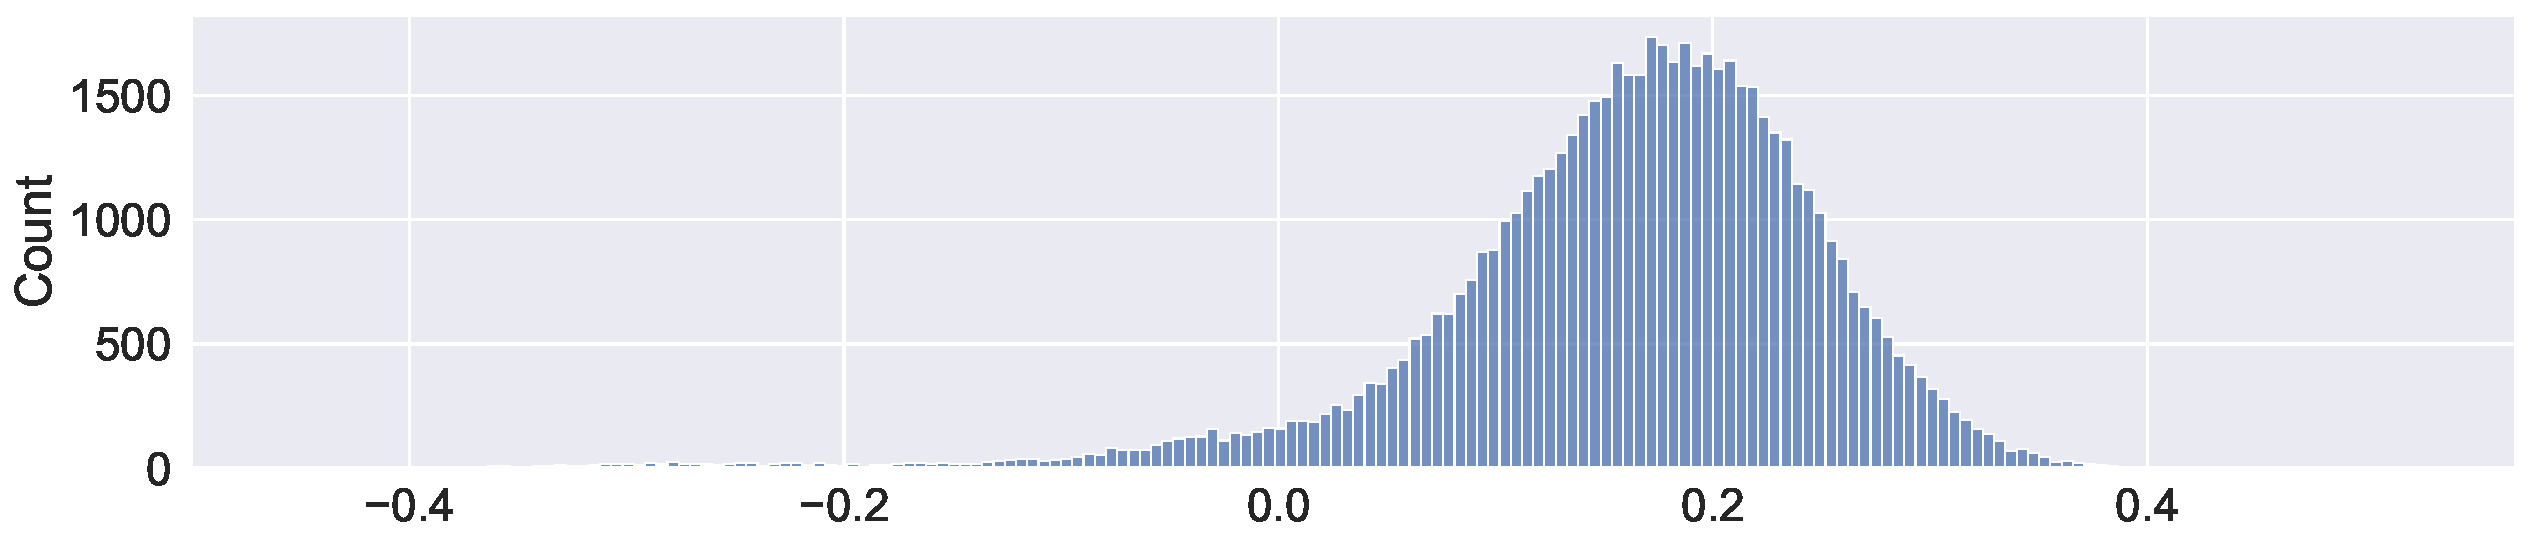
\includegraphics[width=\textwidth]{gfx/probing/labels/sem}
    \caption{Distribution of semantic similarity target scores.}

    \bigskip

    \centering
    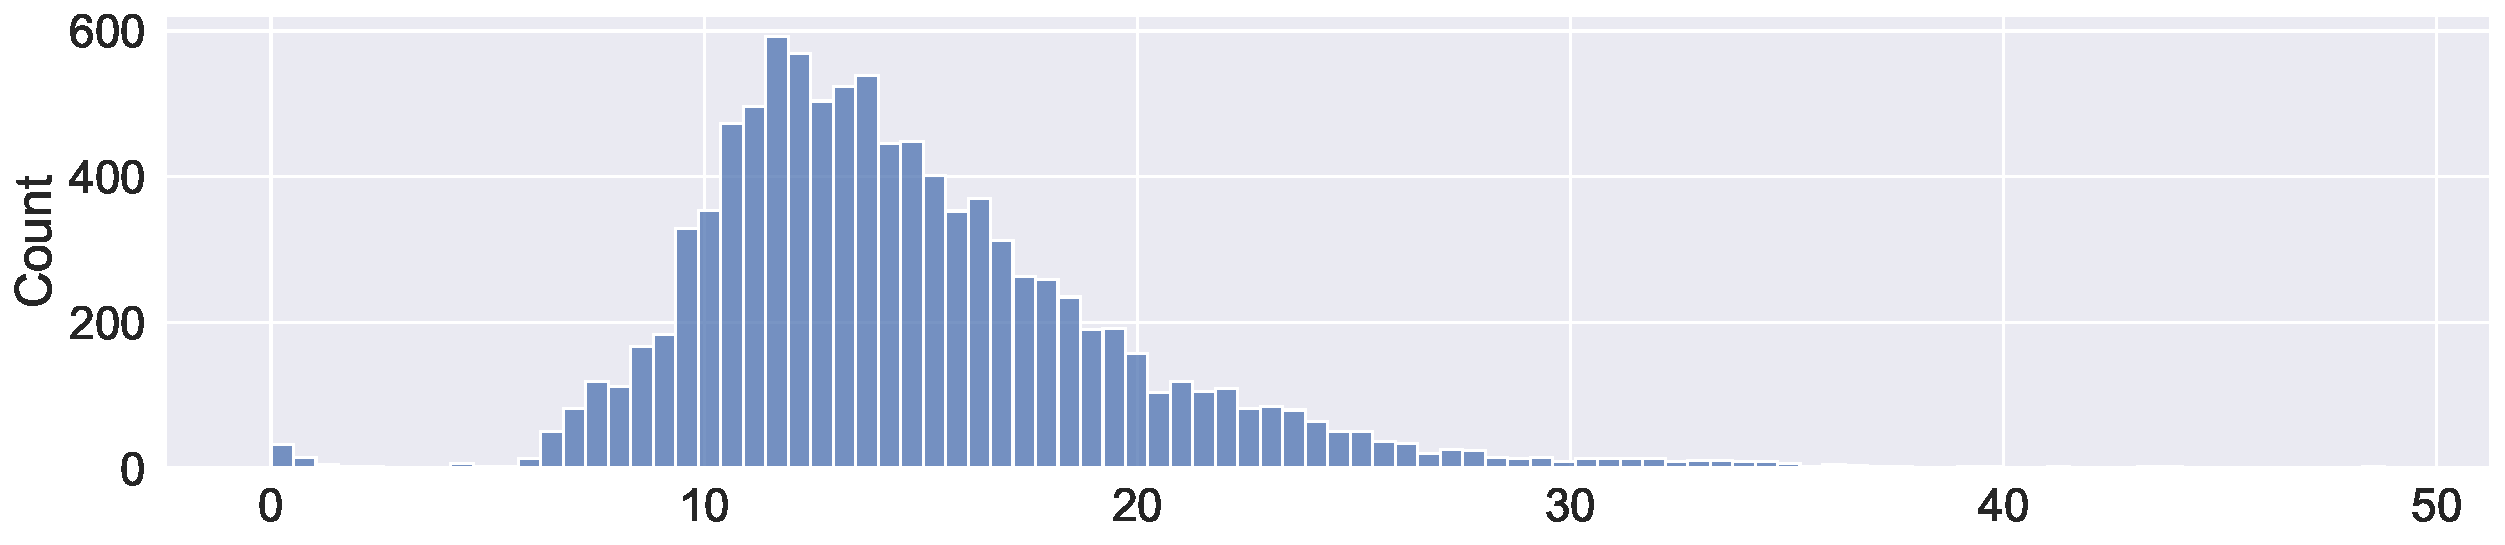
\includegraphics[width=\textwidth]{gfx/probing/labels/bm25}
    \caption{Distribution of BM25 target scores.}

    \bigskip

    \centering
    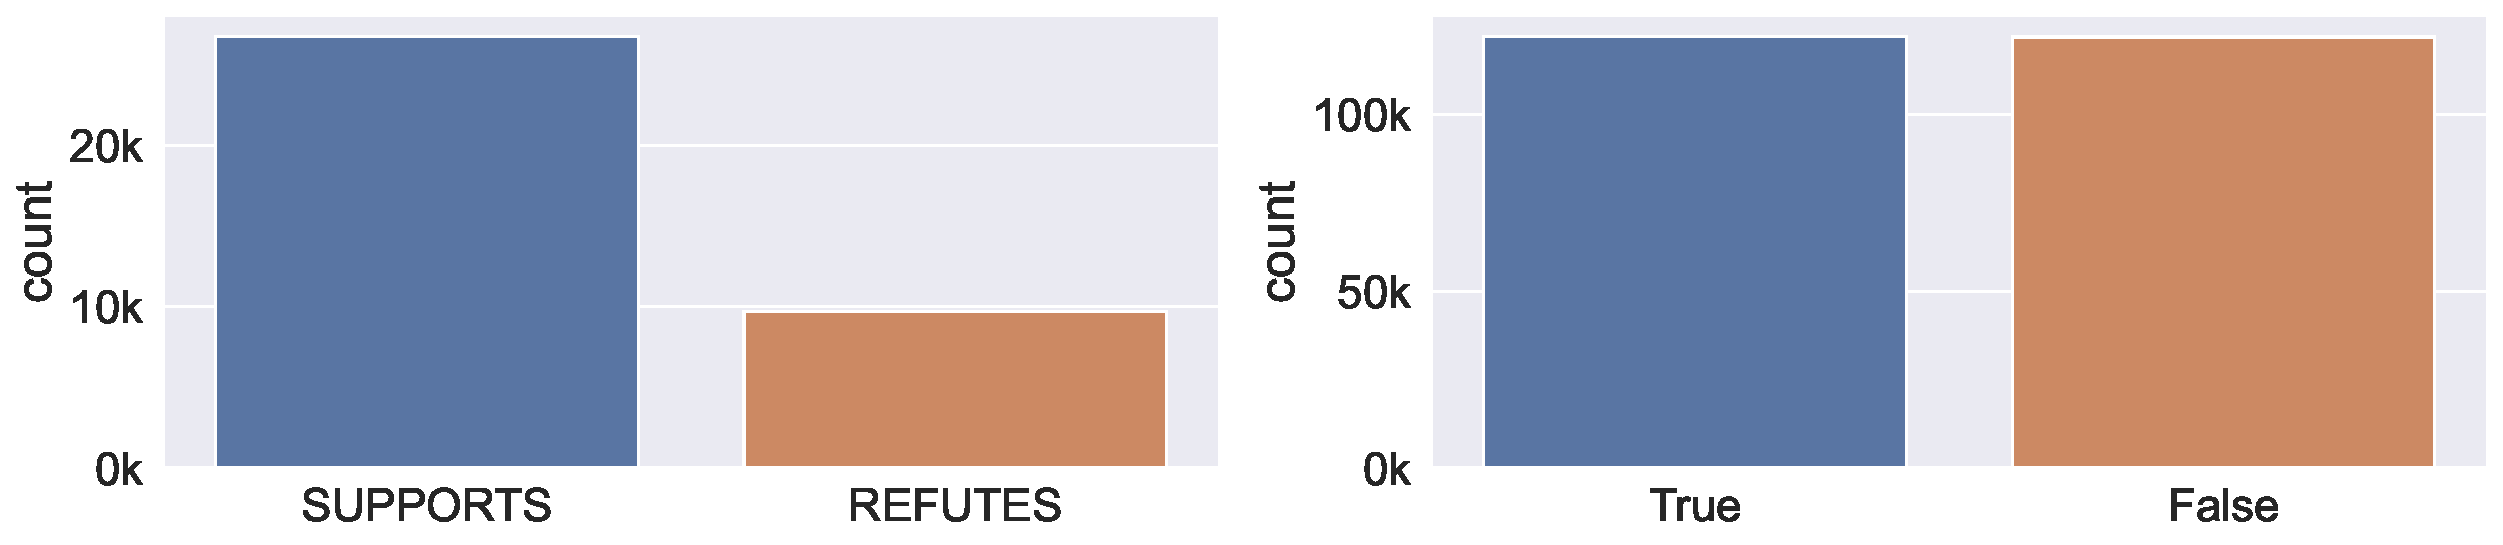
\includegraphics[width=\textwidth]{gfx/probing/labels/fever_coref}
    \caption{Distribution of FEVER and COREF labels. COREF negatives are sampled for each positive.}

    \bigskip

    \centering
    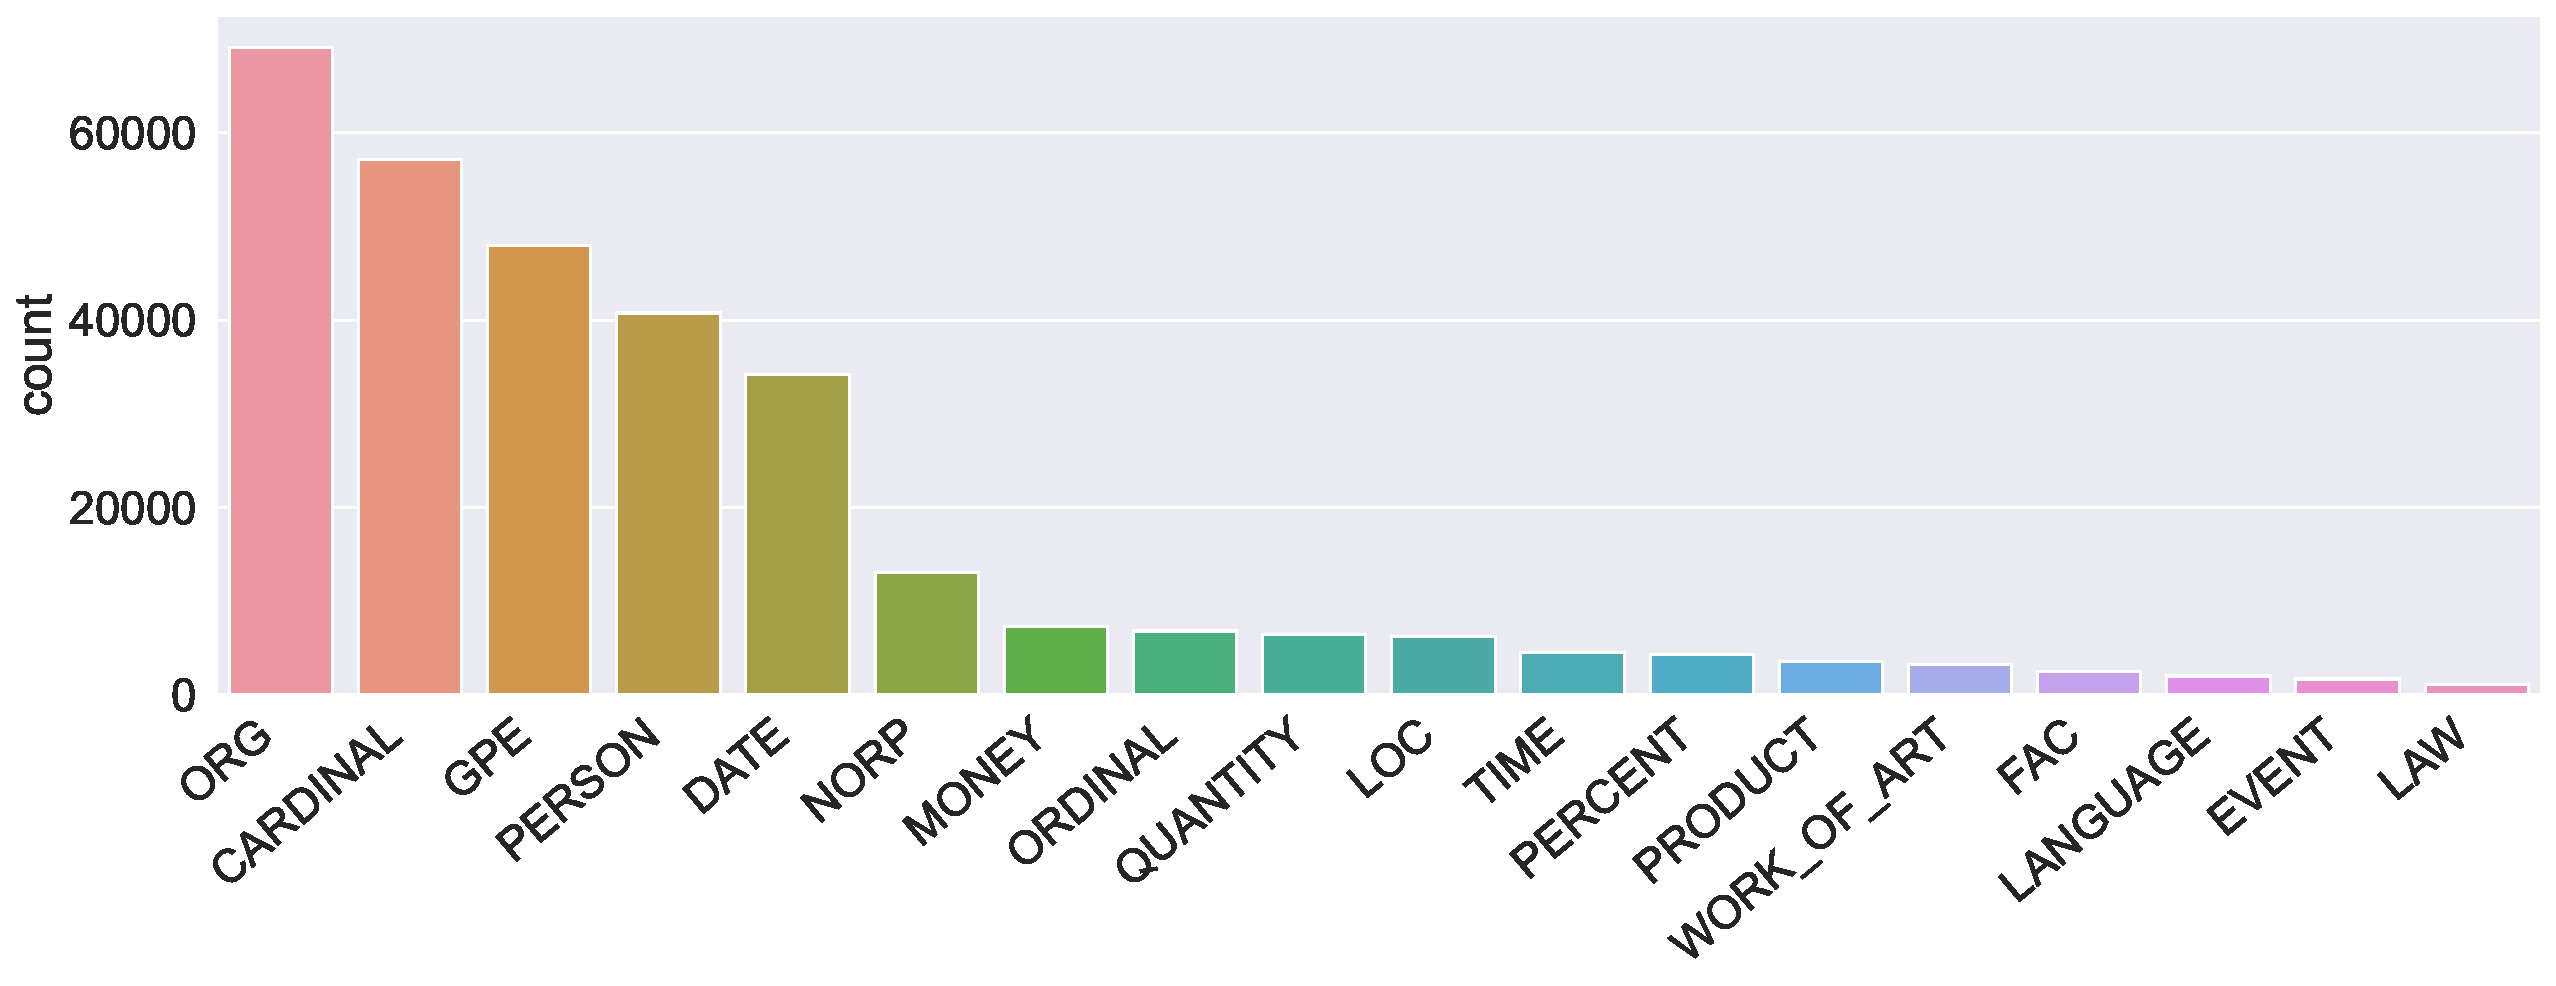
\includegraphics[width=\textwidth]{gfx/probing/labels/ner}
    \caption{Distribution of named entity types in the NER dataset.}

\end{figure}

\chapter{Approach}
\label{chap:approach}

\section{Methodology}
\todo{edge probing graphic}
Our goal is to understand whether certain properties that we expect to be relevant for ranking can be decoded from the hidden representations of a pre-trained transformer model. Further, we want to know to which degree these properties are encoded at different layers within the model.

To test this, we conduct the following experiment: First, we generate a set of datasets $D_{\tx{probing}}=\{D_1, D_2, \dots, D_n \}$, each aimed at predicting a property $Y_i$ that, based on traditional ranking methods, can be considered relevant for ranking. Then, for each dataset, we train a probing classifier $P_i: \R^d \rightarrow \R^c$ on top of the fixed hidden representations $H\lay k = \{h_i\}_{i=1}^N \in \R^{N \times d}$ of subject model $\MSubject$. This procedure is repeated at every layer $k$. Finally, we compare the classifier's performance \todo{performance metric $m(P_i, D_i, H)$?} across layers, to get a relative measure of how task-specific information is distributed throughout $\MSubject$. To further put our measurements into perspective, we also employ a random baseline model $\mathcal{B}$ which is also probed for each task separately.

Following the probing experiments, we then attempt to develop an improved fine-tuning procedure, based on our findings.

\subsection{Task Design}
We propose a set of classification tasks with ranking properties as target variable. In this section we provide a list of the tasks we've chosen and explain the reasoning behind our selection.

\subsubsection{BM25 Prediction}
BM25 (\sect{bm25}) is a well-known text-retrieval method and still considered a first choice when it comes to computational efficiency. As heuristic designed around exact term matching, BM25 quantifies query-document pairs on a symbolic level, without the notion of higher level semantics.

Being able to decode BM25 from BERT embeddings might give a hint on whether exact matching properties like term-frequency or even corpus level statistics like inverted document-frequency are encoded by the neural ranking models.

\subsubsection{Semantic Similarity}
To measure semantic similarity, we compute cosine distance between query and document vectors in the GloVe\cite{pennington2014glove} embedding space:
\begin{equation}
    \tx{Sim}(q, d) = \frac{q^\top d}{||q|| \times ||d||}
\end{equation}
While these dense word representations encode semantics, unlike BERT they are not contextualized, meaning they do not change based on surrounding words in a sentence. In that sense, using semantic similarity as ranking measure may be interpreted as a kind of soft term-matching: Words between query and document that are similar in meaning increase the estimated relevance.

\subsubsection{Coreference Resolution}
Coreference resolution is the task of deciding whether two mentions in a text refer to the same entity. To model coreference we use binary classification over two spans of text in query and document, respectively.

We argue that recognizing whether an entity is shared between query and document can be an important indicator on whether the document is relevant. For instance, knowing that "the us president" in a query refers to "joe biden" in a document is certainly helpful.

\subsubsection{Named Entity Recognition}
Similar to coreference resolution, recognizing entities can be used to match concepts between query and document when performing retrieval. However, in the case of named entity recognition this matching is less restricted, as only entity \ti{types} are considered, instead of specific entities. For example, given the query: "How much PS does a jaguar have?", a document that contains car entities, should be prioritized over one with animal entities.

For our task, we solely test the general ability of the model to encode entities, meaning we treat document and query as a whole and predict entity types of separate text spans.

\subsubsection{Fact Checking}
For fact checking, we leverage the existing FEVER \cite{thorne-etal-2018-fever} dataset. Here, instead of query and document, a claim and evidence text are provided. The goal is to classify whether the evidence supports or refutes the claim. This task requires high level semantic reasoning, making it relevant for more fine-grained ranking, i.e. providing documents that contain \ti{coherent} answers to a query and not only similar ones.

\subsubsection{Relevance Estimation}
Because the TREC2019 dataset provides relevance labels, we can also directly probe what layers contain most information with respect to relevance prediction. This especially becomes interesting when comparing between models tuned for ranking and pure language models.

\subsection{Models}
\subsubsection{Subject Models}
\label{sec:subjects}
Subject of our probing experiments is the pre-trained BERT~\cite{devlin-etal-2019-bert} transformer model. In particular, we use the \ti{bert-base-uncased}\footnote{\url{https://huggingface.co/bert-base-uncased}} variant, which consists of $12$ layers, with $h=12$ attention heads each and a hidden dimension of $d=786$. The model has been trained on BooksCorpus~\cite{7410368} and text passages from English Wikipedia\footnote{\url{https://en.m.wikipedia.org/}}, which consist of 800 million and 2.5 billion words, respectively.

In addition, we probe two fine-tuned \ti{bert-base-uncased} models that we term \ti{bert-msm-passage} and \ti{bert-msm-doc}. Both are trained on datasets from the TREC2019 deep learning track~\cite{DBLP:journals/corr/abs-2003-07820}. While \ti{bert-msm-passage} is trained to predict relevancy of \ti{passages} given a query, \ti{bert-msm-doc} is trained on \ti{document}-level data. Hence, for this purpose we use the TREC2019 passage- and document-level dataset respectively.

Note that all three models share the same architecture and only differ by which datasets they were trained on. Having access to additional versions of \ti{bert-base-uncased} that were fine-tuned specifically for ranking, gives us a way to compare if and how the distribution of information throughout the model changes when being adapted to the new task.

\subsubsection{Probe}
\label{sec:probe}
One problem in probing arises when trying to choose a probe of appropriate complexity \cite{hewitt-liang-2019-designing}. If the classifier is too complex, it might end up modeling new, complex features itself and hence, rely less on the information that is already present in the subject model's representations. On the other hand, if the classifier is too simple, it might not be able to properly decode the information at all.

While there is recent debate on whether more complex models are actually problematic for probing \cite{pimentel-etal-2020-information}, following previous literature \cite{Tenney2019WhatDY,tenney-etal-2019-bert, hewitt-liang-2019-designing} we decide on a simple $2$-layer MLP which, despite its simplicity, is still capable of modeling non-linear relationships.
Specifically, we use the same MLP as \cite{Tenney2019WhatDY}:

\begin{equation}
    \hat{P}(x) = \tx{LayerNorm}(\tx{tanh}(x W^{(0)} + b^{(0)})) W\lay 1 + b^{(1)}
\end{equation}

Where $W\lay 0 \in \R^{|S| d \times d}$,  $W\lay 1 \in \R^{d \times c}$ and $b\lay 0 \in \R^{d}$,  $b\lay 1 \in \R^{c}$ are learned parameters with hidden size $d$ and number of target classes $c$.

Since some tasks require operating over one or multiple spans $S=\{(\tx{start}_i, {end}_i)\}_{i=1}^{|S|}$, we further need to use a pooling mechanism, such that a fixed-length representation can be provided to the probe.
Again, like \cite{Tenney2019WhatDY} we employ the simple attention pooling operator also used in \cite{lee-etal-2017-end, lee-etal-2018-higher}:

\begin{equation}
    \begin{aligned}
         & \alpha_n = \frac{\exp(w^\top h_n)}{\sum_{k=i}^j{\exp(w^\top h_k)}}   \\
         & \tx{pool}(h_i, h_{i+1},\dots, h_j)= \sum_{k=i}^j\alpha_k (W h_k + b)
    \end{aligned}
\end{equation}

Where $w \in \R^{d}$, $W \in \R^{d \times d_{probe}}$, $b \in \R^{d_{probe}}$ are learned parameters which, in the case of multiple spans, are not shared between spans. The pooled span representations are concatenated and passed to the MLP, resulting in the full probe:
\begin{equation}
    P(h_1,\dots, h_N) = \hat{P}\bigg(\bigparallel_{(i, j) \in S}{\tx{pool}(h_i, h_{i+1},\dots, h_j)}\bigg)
\end{equation}

\section{Experimental Setup}
\subsection{Fine-tuning Subject Models}
We fine-tune a \ti{bert-base-uncased} model on both, TREC2019 passage- and document-level datasets (\sect{trec2019}), to obtain ranking subject models \ti{bert-msm-passage} and \ti{bert-msm-doc} (\sect{subjects}), respectively. Each model is trained with a binary cross-entropy objective, for a maximum of $20$ epochs. Early stopping is performed after $3$ epochs, if no increase in validation MAP is observed. For hyperparameters, we keep the default settings suggested by \cite{devlin-etal-2019-bert}, using the Adam optimizer\cite{kingma2014adam} with a learning rate of 1e-5, a mini-batch size of $16$ and linear increase in learning rate over the first $1000$ steps. As BERT uses a fixed set of learned positional embeddings, the input length is limited to $512$ tokens. Hence, we truncate any passages and documents exceeding this maximum length, after applying BERT's word-piece tokenization.

\subsection{Probing}
\section{Evaluation Measures}
\subsection{MDL}
As mentioned in \sect{probe}, selecting a proper size for a probe can be difficult. With a large probing classifier, it becomes unclear whether the property probed for is decoded, or the classifier simply learns the task at hand. One way to address this problem, is to compare how well the classifier performs on randomly initialized baseline representations \cite{zhang-bowman-2018-language}. Further, \cite{DBLP:journals/corr/abs-1909-03368} propose the use of \ti{control tasks}, for which task labels are randomly assigned, and a probe is selected based on the difference in accuracy to the original task. Both approaches however, often do not reflect a large difference in accuracy, when compared to the original representations or task.

As a solution, \cite{voita-titov-2020-information} propose an information theoretic approach for measuring probe performance, instead of accuracy. By recasting learning a probe model to transmitting label data with the least amount of bits, a new measure can be applied: The \ti{minimum description length} (MDL) required for transmitting the task labels, given the probed representations. Not only does MDL measure the probe's predictive performance, it also takes into account the amount of effort for achieving this performance, manifesting in model size or amount of training data required.

Since \cite{voita-titov-2020-information} find that MDL is a more representative and also reliable measure than accuracy, we also choose it as preferred method for measuring probe performance. To compute MDL, we use the online code definition \cite{Rissanen1984UniversalCI}.
For this, the probing dataset $D=\{(x_i, y_i)\}_{i=1}^n$ is divided into timesteps $1=t_0 < t_1 < \ldots < t_S = n$. After encoding block $t_0$ with a uniform code, for each following timestep a probing model $P_{\theta_i}$ is trained on the samples $(1, \ldots, t_i)$ and used to predict over data points $(t_i + 1,\ldots, t_{i + 1})$. The full MDL is then computed as sum over the codelengths of each $P_{\theta_i}$ and the uniform encoding of the first block:

\begin{equation}
    \begin{aligned}
         & \tx{MDL}(y_{1:n} | x_{1:n}) = t_1 \log_2 c                                        \\
         & - \sum_{i=1}^{S-1} \log_2 P_{\theta_i}(y_{t_i + 1:t_{i+1}} | x_{t_i + 1:t_{i+1}})
    \end{aligned}
\end{equation}

where $c$ is the number of target classes.
Following \cite{voita-titov-2020-information}, we choose timesteps at $0.1$, $0.2$, $0.4$, $0.8$, $1.6$, $3.2$, $6.25$, $12.5$, $25$, $50$ and $100$ percent of the dataset.

\subsection{Compression}
Because MDL depends on the number of targets in a probing dataset, it is not reasonable to directly compare it between different tasks. A common way to turn MDL into a relative measure, is by computing \ti{compression}. Compression divides the codelength that would result from a uniform encoding by MDL:

\begin{equation}
    \tx{compression} = \frac{n \log_2(c)}{\tx{MDL}(y_{1:n} | x_{1:n})}
\end{equation}

This means compression is a measure of how much easier it is for the probe to decode a property from the probed representations, or in other words how well they encode the task labels.
\subsection{Accuracy}
\subsection{Ranking}
\subsubsection{MAP}
\subsubsection{MRR}
\subsubsection{NDCG}
\subsubsection{Precision}


\chapter{Results}
\label{chap:results}

- old plots
- task to layer to map plot

\chapter{Conclusion}
\label{chap:conclusion}

\section{Future Work}


\chapter*{Plagiarism Statement}
\addcontentsline{toc}{chapter}{Plagiarism Statement}
\vfill
\mbox{} \\
{\large I hereby confirm that this thesis is my own work and that I have documented all sources used.}
\newline
\mbox{} \\
Hannover, \handindate \\
\vspace{4cm}
\hrule
\vspace{0.5cm}
$\qquad$(Fabian Beringer)

\listoffigures
\addcontentsline{toc}{chapter}{\listfigurename}
\listoftables
\addcontentsline{toc}{chapter}{\listtablename}
\clearpage
\phantomsection
\addcontentsline{toc}{chapter}{Bibliography} 
\printbibliography
\end{document}